\documentclass[9pt,a4paper,twocolumn,twoside]{rho-class/rho}

% --- 1. Idioma y matemáticas básicas ---
\usepackage[spanish,es-nodecimaldot,es-noindentfirst,es-noshorthands]{babel}

% --- 2. EL TRUCO DE MAGIA (BIEN ESCRITO) ---
% Borramos los comandos problemáticos usando su nombre exacto interno
\expandafter\let\csname not=\endcsname\relax
\expandafter\let\csname not<\endcsname\relax
\expandafter\let\csname not>\endcsname\relax

% Ahora ya podemos cargar la fuente moderna sin que explote
\usepackage{fontspec}
\usepackage{unicode-math}

% --- 3. Bibliografía ---
\addbibresource{rho.bib}

% --- 4. Datos del Informe ---
\title{Estudio de la vida media y conversión interna del Ba$^{137\text{m}}$}
\author{Edgar Fernández Vigil}
\affil{Física - Facultad de Ciencias - Universidad de Oviedo}
\dates{\today}
\journalname{TEIII - Práctica de Laboratorio}
\journal{Vida media y conversión interna del Ba$^{137\text{m}}$}

% --- 5. Resumen ---
\begin{abstract}
\noindent
En este artículo detallamos el estudio experimental del decaimiento radiactivo del Bario-137 metaestable. Primero, extraemos el Bario de una muestra de Cesio-137 mediante un proceso químico. Después, medimos la actividad de este Bario en función del tiempo usando un detector de centelleo, comprobando que cae de forma exponencial y calculando su vida media. Además, estudiamos su espectro de energías para ver cuántas veces ocurre la conversión interna en vez de la emisión gamma, y usamos la actividad de la pastilla original para intentar estimar hace cuántos años se fabricó.
\end{abstract}

% ----------------------------------------------------------
\begin{document}

    \maketitle
    \thispagestyle{firststyle}

\section{Introducción y motivación}

\rhostart{E}n esta práctica vamos a estudiar de primera mano cómo funciona el decaimiento radiactivo, que como sabemos es un proceso puramente aleatorio regido por la conocida ley exponencial $N(t)=N_{0}e^{-\lambda t}$. Para ello, nos centraremos en analizar el Cesio-137 ($^{137}\text{Cs}$). Este isótopo decae emitiendo una partícula $\beta$ y se transforma en Bario-137 metaestable ($^{137m}\text{Ba}$).

Lo interesante de este Bario metaestable es que le sobra energía (unos 661.7 keV) y necesita soltarla para quedarse en su estado fundamental estable. Además, lo hace rapidísimo: su vida media es de apenas dos minutos y medio. Lo más normal es que libere esa energía disparando un fotón $\gamma$ sin más. Sin embargo, a veces ocurre un fenómeno alternativo muy curioso llamado conversión interna.

En esta conversión interna, en lugar de emitir el fotón $\gamma$, el núcleo le pasa la energía directamente a uno de los electrones más internos del átomo (suele ser de la capa K) y lo expulsa. Al quedarse ese hueco libre, otro electrón de las capas externas cae para rellenarlo, emitiendo en el proceso un rayo X característico de unos 32.2 keV. 

Durante nuestra sesión en el laboratorio, usaremos un generador de isótopos para extraer el Bario, sacándolo de su "padre" el Cesio. Así, podremos ponerlo bajo el detector para ver en tiempo real cómo decae su actividad, calcular su vida media y, estudiando sus picos de energía, descubrir qué porcentaje exacto de las veces ocurre esta conversión interna.

\section{Objetivos}

La finalidad general de esta práctica es familiarizarnos con la dinámica radiactiva y el uso de la espectrometría gamma. Para ello buscaremos:

\begin{itemize}
    \item \textbf{Comprender el decaimiento radiactivo:} Afianzar los conceptos de vida media y constante de desintegración ($\lambda$), estudiando de forma práctica su caída exponencial.
    \item \textbf{Extraer nucleidos radiactivos:} Entender cómo funciona el proceso químico para extraer el isótopo hijo ($^{137m}\text{Ba}$) de su isótopo padre ($^{137}\text{Cs}$).
    \item \textbf{Determinar la vida media del estado metaestable:} Medir la actividad de la muestra extraída en función del tiempo para obtener su curva de desintegración y calcular cuánto tarda en decaer.
    \item \textbf{Cuantificar la conversión interna:} Estimar la tasa o fracción de conversión interna ($F$) calculando la relación matemática entre el área del pico de rayos X y el área del pico de rayos $\gamma$.
    \item \textbf{Aplicar técnicas de datación:} Utilizar la actividad medida de la fuente original para intentar calcular la antigüedad de la pastilla radiactiva de nuestro laboratorio.
\end{itemize}

\section{Dispositivo Experimental}

Para llevar a cabo las mediciones, montamos un dispositivo que consta del siguiente equipamiento:

\begin{itemize}
    \item \textbf{Detector de centelleo:} Cristal de NaI(Tl) de $38.1 \times 50.8$ mm acoplado a un tubo fotomultiplicador (PMT) y conectado a una fuente de alta tensión (HV). 
    \item \textbf{Analizador Multicanal (MCA):} Dispositivo encargado de procesar los pulsos del detector para discriminar las energías y generar el espectro. 
    \item \textbf{Generador de isótopos:} Kit de extracción que contiene una pastilla madre de $^{137}\text{Cs}$, del cual extraemos el $^{137\text{m}}\text{Ba}$ haciéndole pasar una solución salina acidulada (0.9\% NaCl en 0.04M HCl). 
    \item \textbf{Software de análisis:} Programa PHYWE Measure instalado en el PC para grabar los espectros y registrar las cuentas a lo largo del tiempo. 
\end{itemize}

\section{Procedimiento Experimental}

Procedimos a realizar la práctica dividiendo la toma de datos en varias etapas:

\subsection{Extracción del isótopo metaestable}
Para extraer el Bario usamos el generador de isótopos. Simplemente hicimos pasar la solución salina por la cápsula y, como el Cesio se queda atrapado dentro, logramos sacar únicamente el $^{137\text{m}}\text{Ba}$. En cuanto tuvimos la muestra, la llevamos rápido al detector para empezar a medir antes de que decayera.
\subsection{Medición del decaimiento temporal}
A continuación, colocamos la muestra recién extraída bajo el detector de centelleo. Configuramos el software para tomar medidas automáticas en intervalos de tiempo fijos durante unos 15 minutos. De esta forma, fuimos registrando cómo disminuía la tasa de conteo a medida que el Bario decaía a su estado estable.

\subsection{Espectroscopía y conversión interna}
Para estudiar la conversión interna, pusimos la pastilla madre original bajo el detector y registramos su espectro de energías completo. Identificamos los picos correspondientes a los rayos $\gamma$ y a los rayos X y medimos las áreas bajo la curva de cada uno para poder calcular sus probabilidades relativas.

\subsection{Análisis de datos y datación}
Por último, para analizar los datos, medimos también la radiación de fondo ambiental del laboratorio para poder restársela a nuestras medidas. Realizamos ajustes matemáticos para extraer la constante de desintegración y usamos la actividad total de la pastilla madre para intentar deducir cuántos años hace que la fabricaron.

\section{Resultados y Discusión}

\subsection{Obtención de los espectros}

\subsubsection*{Sin muestra (espectro de fondo)}
En primer lugar, realizamos una medición en ausencia de muestra para caracterizar el fondo radiactivo del laboratorio. 

\begin{figure}[htbp]
    \centering
    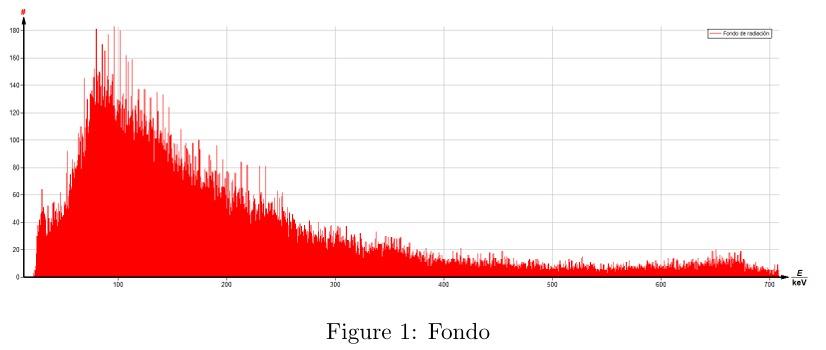
\includegraphics[width=\linewidth]{img/fondo.jpeg}
    \caption{Espectro energético de la radiación de fondo ambiental.}
    \label{fig:espectro_fondo}
\end{figure}

Como observamos en la Figura \ref{fig:espectro_fondo}, el espectro de fondo presenta una distribución continua generada fundamentalmente por la radiación de frenado (\textit{Bremsstrahlung}) al interactuar la radiación cósmica con los materiales del entorno. Sobre este continuo destacan un pico en torno a 80 keV (atribuible a las desintegraciones del Radón natural y a la fluorescencia del blindaje de plomo) y un pico muy tenue en 32 keV, correspondiente a los rayos X del Yodo al excitarse el propio cristal del detector.

\subsubsection*{Con muestra}
A continuación, colocamos la pastilla madre radiactiva sobre el centellador. En la Figura \ref{fig:espectro_muestra} identificamos los fenómenos esperados:

\begin{figure}[htbp]
    \centering
    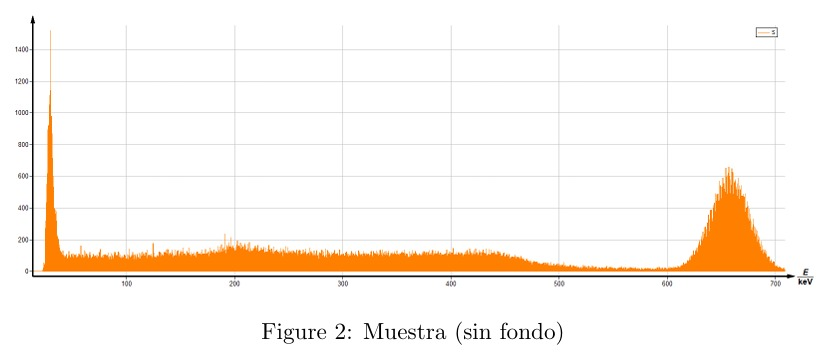
\includegraphics[width=\linewidth]{img/muestra.jpeg}
    \caption{Espectro bruto de la muestra de $^{137}\text{Cs}/^{137m}\text{Ba}$.}
    \label{fig:espectro_muestra}
\end{figure}

\begin{itemize}
    \item \textbf{Fotopico de 662 keV:} Corresponde a la desexcitación $\gamma$ de los núcleos de Bario hacia su estado fundamental.
    \item \textbf{Meseta Compton:} Generada por los fotones que rebotan en los electrones del detector y escapan sin depositar toda su energía.
    \item \textbf{Pico de retrodispersión (\textit{Backscattering}):} En torno a 200 keV, originado por fotones que rebotan en la mesa o el blindaje y entran al detector con menos energía.
    \item \textbf{Pico de rayos X a 32.2 keV:} Causado por el proceso de conversión interna al reestructurarse la corteza electrónica tras la eyección de un electrón de la capa K.
\end{itemize}

\subsection{Estimación de la tasa de conversión interna (\texorpdfstring{$F$}{F})}

Para cuantificar matemáticamente esta conversión interna, sustrajimos el espectro de fondo a nuestra medida y ajustamos una recta en el valle Compton para poder aislar el área neta de los picos. El resultado limpio se observa en la Figura \ref{fig:espectro_Sprima}.

\begin{figure}[htbp]
    \centering
    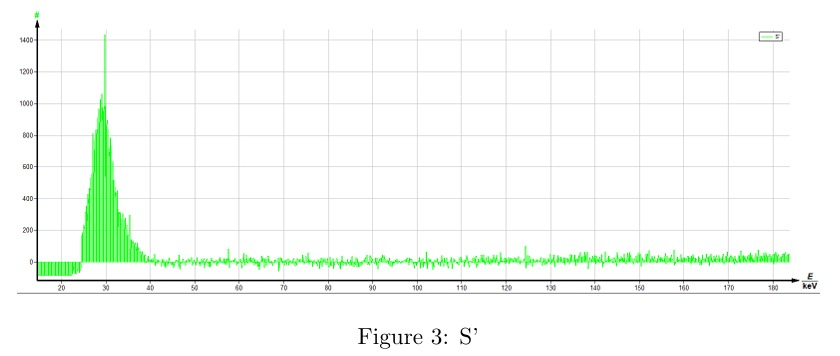
\includegraphics[width=\linewidth]{img/figura3.jpeg}
    \caption{Espectro depurado tras la sustracción del fondo y el continuo.}
    \label{fig:espectro_Sprima}
\end{figure}

A partir de las áreas de ambos picos (Rayos X y emisión $\gamma$), determinamos empíricamente la fracción de conversión interna:
\vspace{0.2cm}
\begin{equation*}
    F = 0.087 \pm 0.004
\end{equation*}
\vspace{0.2cm}

Este resultado es sumamente próximo al valor de referencia teórico ($F_{ref} = 0.09128 \pm 0.00042$). La pequeña diferencia entra perfectamente dentro del margen de error sistemático introducido al seleccionar manualmente con el ratón el rango de integración de los canales en el software.

\subsection{Medida de la vida media del \texorpdfstring{$^{137m}\text{Ba}$}{Ba-137m}}

\subsubsection*{Evolución de la actividad de la muestra matriz}
Al medir la evolución de la pastilla de Cesio intacta en función del tiempo (Figura \ref{fig:muestra_tiempo}), comprobamos que la actividad total se mantiene completamente plana y constante. Esto se debe a que la vida media del Cesio-137 ($\approx 30$ años) garantiza que siga generando Bario al mismo ritmo que este decae (equilibrio secular).

\begin{figure}[htbp]
    \centering
    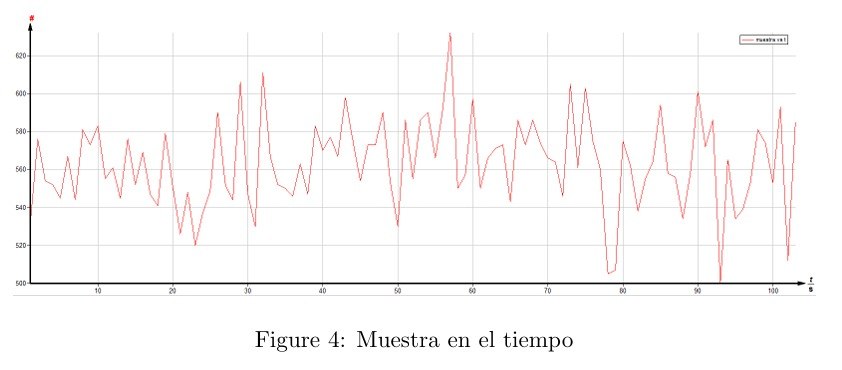
\includegraphics[width=\linewidth]{img/muestra-tiempo.jpeg}
    \caption{Evolución temporal de las cuentas en la muestra matriz.}
    \label{fig:muestra_tiempo}
\end{figure}

Al agrupar estas cuentas temporalmente estables, el comportamiento puramente aleatorio de las desintegraciones nos devuelve una distribución de probabilidad en forma de campana de Gauss (Figura \ref{fig:gaussiana}), dándonos una actividad media para nuestra pastilla de $\mu = 563 \pm 2$ cuentas/s y una desviación de $\sigma = 22 \pm 2$ cuentas/s.

\begin{figure}[htbp]
    \centering
    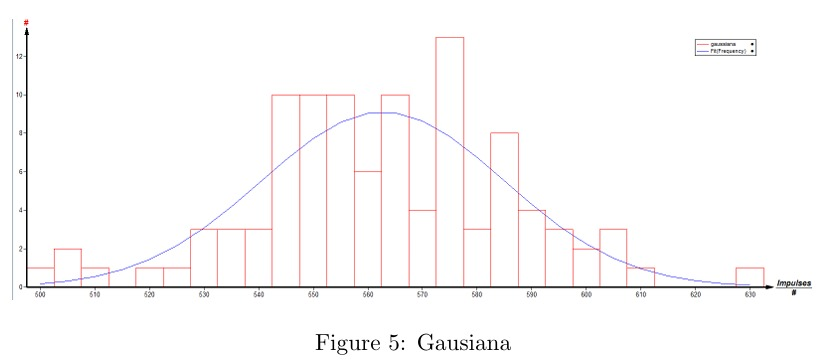
\includegraphics[width=\linewidth]{img/gausiana.jpeg}
    \caption{Ajuste gaussiano de la actividad total de la muestra.}
    \label{fig:gaussiana}
\end{figure}

\subsubsection*{Evolución del fondo en el tiempo}
De forma paralela, verificamos que el fondo ambiental oscila estadísticamente pero no sufre caídas ni subidas netas durante el tiempo de estudio, como se aprecia en la Figura \ref{fig:fondo_tiempo}.

\begin{figure}[htbp]
    \centering
    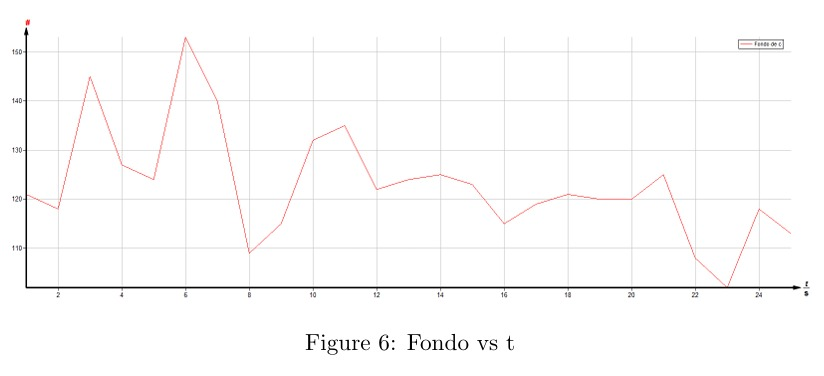
\includegraphics[width=\linewidth]{img/fondo-vs-tiempo.jpeg}
    \caption{Evolución temporal constante de la actividad del fondo radiactivo.}
    \label{fig:fondo_tiempo}
\end{figure}

\subsubsection*{Evolución de la muestra extraída}
Para poder medir verdaderamente la vida media del isótopo hijo $^{137m}\text{Ba}$, llevamos la muestra radiactiva que acabábamos de extraer al detector.

\begin{figure}[htbp]
    \centering
    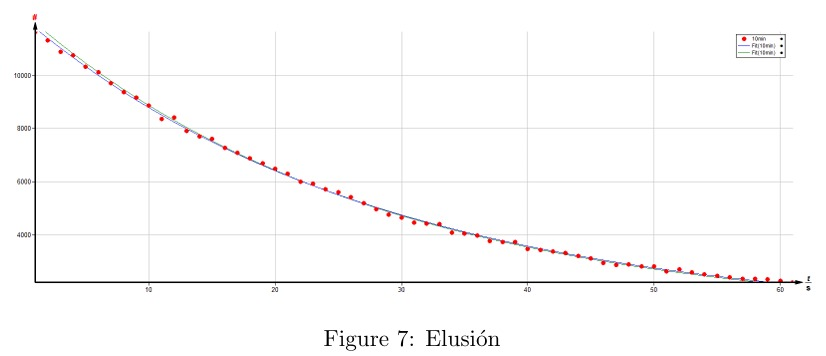
\includegraphics[width=\linewidth]{img/elusion.jpeg}
    \caption{Decaimiento exponencial de la actividad del $^{137m}\text{Ba}$ extraído.}
    \label{fig:elusion}
\end{figure}

La Figura \ref{fig:elusion} exhibe la fortísima caída de actividad según el modelo exponencial $A(t) = a e^{-bt} + c$. Al realizar el ajuste sobre los datos experimentales, obtuvimos una constante de desintegración $b = (3.61 \pm 0.18) \times 10^{-3} \text{ s}^{-1}$. A partir de este valor, calculamos su periodo de semidesintegración:
\vspace{0.2cm}
\begin{equation*}
    t_{1/2} = \frac{\ln(2)}{b} = 3.2 \pm 0.2 \text{ min}
\end{equation*}
\vspace{0.2cm}

Este valor es ligeramente superior al tiempo de referencia ($2.551$ min). Físicamente, esto tiene mucho sentido y se explica por el "tiempo muerto" del detector: en los primeros segundos de la medida, la muestra extraída es tan radiactiva que el centellador se satura y no da abasto para procesar todos los pulsos, perdiendo cuentas. Esto hace que la curva parezca más plana al principio y alargue artificialmente el cálculo de la vida media.

\subsection{Determinación de la antigüedad de la muestra}

Para el apartado final de la datación, partimos de la actividad medida en nuestra campana de Gauss, $A = 563 \pm 2$ Bq.
Como el detector no envuelve por completo la muestra, tenemos que aplicar un factor de corrección geométrica (asumiendo que situamos la pastilla a una distancia $d = 6.0 \pm 0.1$ cm de un detector cuyo radio es $x = 1.90 \pm 0.05$ cm). La actividad teórica total a cuerpo completo ($4\pi$) nos da:
\vspace{0.2cm}
\begin{equation*}
    A' = A \frac{4\pi d^2}{\pi x^2} = (22.3 \pm 1.4) \times 10^3 \text{ Bq}
\end{equation*}
\vspace{0.2cm}

Empleando la ley de decaimiento radiactivo con la actividad inicial de fábrica ($A_0 = 370$ kBq) y la constante temporal $\tau = 43.35$ años, despejamos el tiempo que ha transcurrido. (Asumimos también que la emisión $\gamma$ es representativa del $\approx 95\%$ de las desintegraciones totales del Cesio):
\vspace{0.2cm}
\begin{equation*}
    t = -\tau \ln\left(\frac{A'}{0.95 A_0}\right) = 119 \pm 3 \text{ años}
\end{equation*}
\vspace{0.2cm}

Como es obvio, este resultado es gigantesco y difiere completamente de la edad real de la muestra de laboratorio. Esta enorme desviación radica en el fracaso de nuestra hipótesis inicial: aproximar la pastilla a una "fuente puntual ideal" es incorrecto. La geometría real del plástico que la envuelve y la autoabsorción de la propia muestra provocan que muchos fotones se queden atascados dentro y nunca lleguen al detector. Al registrar muchas menos cuentas de las teóricas, las matemáticas nos devuelven una muestra muchísimo más antigua y desgastada de lo que realmente es.

\section{Conclusiones}

Esta práctica nos ha servido para comprobar en el laboratorio cómo funciona el decaimiento radiactivo exponencial. Al analizar el espectro de energías del Bario, pudimos identificar claramente el efecto Compton y la radiación de frenado, y además calculamos que la conversión interna ocurre con una fracción $F = 0.087 \pm 0.004$, lo que cuadra bastante bien con el valor teórico.

Al extraer el Bario, medimos que su vida media es de $t_{1/2} = 3.2 \pm 0.2$ min. Aunque es un poco más alta con respecto al valor de referencia, esto nos ha venido genial para comprobar los efectos del "tiempo muerto" del equipo, que pierde algunas cuentas al principio cuando la muestra es demasiado radiactiva.

Por último, cuando intentamos datar la muestra de Cesio, nos dio una antigüedad de $119 \pm 3$ años. Este resultado físicamente imposible es una gran lección: nos demuestra que tratar una muestra real como si fuera un punto ideal que emite en todas direcciones es un error muy grave. La propia pastilla absorbe un montón de radiación y hace que detectemos menos cuentas de las que deberíamos, sobrestimando muchísimo los años que han pasado.

\newpage
\appendix
\section{Propagación de incertidumbres}

Las incertidumbres reportadas en el cuerpo de este informe han sido calculadas de manera analítica mediante el método general de derivadas parciales, propagando los márgenes de error estadísticos (Poisson) o instrumentales de cada magnitud. A continuación detallamos las expresiones empleadas.

\subsection*{1. Tasa de conversión interna (F)}
La probabilidad de conversión depende del área integrada bajo el fotopico de rayos X ($A_K$) y la emisión gamma ($A_\gamma$). La propagación de su desviación se define por:
\vspace{0.2cm}
\begin{equation*}
    \delta F = \sqrt{ \left( \frac{\partial F}{\partial A_K} \cdot \delta A_K \right)^2 + \left( \frac{\partial F}{\partial A_\gamma} \cdot \delta A_\gamma \right)^2 }
\end{equation*}
\vspace{0.2cm}

\subsection*{2. Actividad actual (A) y Vida Media ($t_{1/2}$)}
La actividad detectada se extrae de la media $\mu$ de nuestra distribución gaussiana. Para considerar el efecto del fondo ambiental ($Fondo$), la incertidumbre en la tasa neta asume la combinación en cuadratura de ambos parámetros:
\vspace{0.2cm}
\begin{equation*}
    \delta A = \sqrt{ \left( \frac{\partial A}{\partial \mu} \cdot \delta \mu \right)^2 + \left( \frac{\partial A}{\partial Fondo} \cdot \delta Fondo \right)^2 }
\end{equation*}
\vspace{0.2cm}

En el caso del decaimiento temporal, la vida media está gobernada por la constante $b$ deducida del ajuste exponencial. Tomando el error absoluto que nos devuelve Python para dicho ajuste ($\delta b$), la propagación es directa:
\vspace{0.2cm}
\begin{equation*}
    \delta t_{1/2} = \left| \frac{\partial t_{1/2}}{\partial b} \cdot \delta b \right| = \frac{\ln(2)}{b^2} \delta b
\end{equation*}
\vspace{0.2cm}

\subsection*{3. Antigüedad de la muestra ($t$)}
La datación se fundamenta en la actividad extrapolada al ángulo sólido total. Primero, evaluamos la incertidumbre de dicha actividad corregida ($A'$) ponderando los errores de la regla en la distancia ($d$) y el radio de la ventana del detector ($x$):
\vspace{0.2cm}
\begin{equation*}
    \delta A' = \sqrt{ \left( \frac{\partial A'}{\partial A} \cdot \delta A \right)^2 + \left( \frac{\partial A'}{\partial d} \cdot \delta d \right)^2 + \left( \frac{\partial A'}{\partial x} \cdot \delta x \right)^2 }
\end{equation*}
\vspace{0.2cm}

Dado que la ecuación temporal que hemos empleado es $t = -\tau \ln\left(\frac{A'}{0.95 A_0}\right)$, propagamos directamente la incertidumbre de la vida media tabular ($\delta \tau$). Con todo ello, la desviación temporal global en la edad de la pastilla la calculamos finalmente como:
\vspace{0.2cm}
\begin{equation*}
    \delta t = \sqrt{ \left( \frac{\partial t}{\partial A'} \cdot \delta A' \right)^2 + \left( \frac{\partial t}{\partial \tau} \cdot \delta \tau \right)^2 }
\end{equation*}
\vspace{0.2cm}

\end{document}